\documentclass{article}
\usepackage[margin=.9in]{geometry}
\usepackage{xcolor}
\usepackage{subcaption}
\usepackage{amsmath}
\usepackage{amssymb}
\usepackage{float}
\usepackage{listings}
\usepackage{natbib}
\usepackage{booktabs}
\usepackage{listings}
\lstset{
basicstyle=\small\ttfamily,
breaklines=true,
frame=single,
language=Python,
numberstyle=\tiny,
showstringspaces=false
}
\setlength{\parindent}{0pt}
\setlength{\parskip}{\baselineskip}
\definecolor{mycolor}{rgb}{0.1, 0.1, 0.5}
\title{\textcolor{mycolor}{\textbf{{\huge Development and Implementation of a Low-Cost Electrochemistry Lab Kit for Educational Outreach}}}}
\author{Student: Christopher Hunt \\ Mentor: Dr. Kelsey Stoerzinger}
\date{}
\usepackage{graphicx}
\usepackage{fancyhdr}


\begin{document}
\pagestyle{fancy}
\fancyhf{}
\rfoot{}
\lfoot{Christopher Hunt}
\lhead{Development and Implementation of a Low-Cost Electrochemistry Lab Kit for Educational Outreach}
\rhead{\thepage}
\maketitle


\subsection*{Abstract}


This report presents a comprehensive review and comparative study of four different potentiostat designs: The Meloni Design, CheapStat, PaqariStat, and SimpleStat. Each design was evaluated based on the criteria of design complexity, functional efficacy, and educational accessibility. After careful consideration, the Meloni Design was selected as the foundational blueprint for our project due to its simplicity, functionality, and educational value. Modifications were made to the Meloni Design in an attempt to enhance the precision of the control signal and simplify the implementation of the hardware design. Despite these improvements, persistent issues were encountered with accurately measuring the output current at the working electrode. While the expected current range was approximately between -2.5 mA to 2.5 mA, our design produced readings that fluctuated between 0 mA and 0.6 mA. These findings underscore the challenges and complexities involved in DIY potentiostat design. Future research will focus on addressing these limitations to improve the performance and reliability of our educational potentiostat.


\subsection*{Introduction}
Electrochemical research holds immense potential to address challenges in energy sustainability and environmental conservation. This field encompasses work on renewable energy generation, energy storage, and environmental remediation, among others. A cornerstone for propelling advancements in these areas is educating the next generation of engineers and scientists. However, the significant costs associated with essential instrumentation, coupled with a lack of educational resources, present considerable hurdles.


At the heart of electrochemical research lies the potentiostat; an instrument fundamental to a variety of experimental methods. Commercial potentiostats often retail for over a thousand dollars, which is a price point that restricts educational opportunities and limits the pursuit of electrochemical innovation.


An increasing number of researchers have leveraged the rising accessibility of affordable microcontrollers, like the Arduino Uno, to develop low-cost potentiostats [Cook 2020]. While these economical devices may not yet match the capabilities of their commercial counterparts, they serve as invaluable educational tools. Still a gap exists between the research and the standardization of design for academic use. Literature explored in this report has shown designs all meeting benchmark testing, however, these projects remain difficult to implement in a high school or undergraduate setting. By introducing electrochemical techniques to students and resource-constrained communities, these low-cost potentiostats facilitate learning and stimulate innovation, despite financial limitations.


\subsection*{Literature Review}
Four potentiostat designs were reviewed: The Meloni Design [Meloni 2016], CheapStat [Rowe 2011], PaqariStat [Cordova-Huaman 2021], and SimpleStat [Butterworth 2019]. These designs will be evaluated against specific criteria that align with our ambition to enhance education and outreach in electrochemical engineering. These criteria include: design complexity, functional efficacy, and educational accessibility.
\begin{figure}[H]
\centering
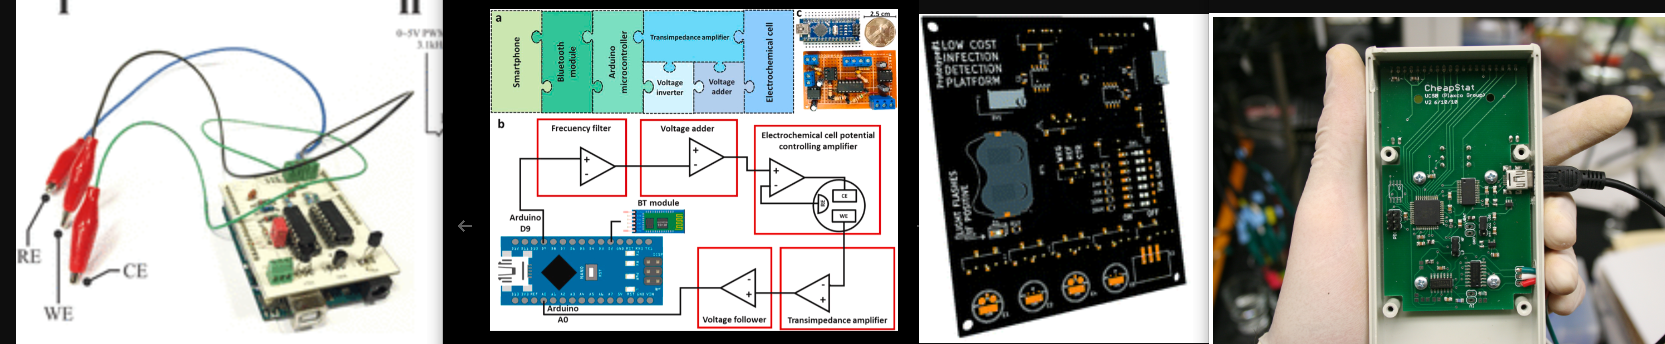
\includegraphics[width=1\linewidth]{review.png}
\caption{Left to Right: Meloni Design, PaqariStat, SimpleStat, CheapStat}
\end{figure}
\subsubsection*{Design Complexity}
Potentiostat design complexity is a critical factor that influences both the user experience and the device's functional range. Among the four studied designs, two design approaches are discernible: the Arduino-based designs (the Meloni design and Paqari Stat) and the Integrated Chip (IC) based designs (Cheapstat and Simplestat). Each design's complexity is influenced by the hardware architecture and software implementation.


\subsubsection*{Hardware Architecture}
The Meloni design and the Paqari Stat employ an Arduino Uno microcontroller as the backbone of their design. Their hardware architectures are modular, composed of three primary units: a Digital to Analog Converter (DAC)/signal converter, a control amplifier, and a transimpedance amplifier. This modular design approach can facilitate problem isolation, making it easier to diagnose and resolve hardware issues. However, there are slight differences between these two designs; while the Meloni design utilizes a counter electrode to measure output current, the Paqari Stat uses the working electrode for this purpose. This difference might impact the overall measurement accuracy, stability, and noise performance of the system.


On the other hand, Cheapstat and Simplestat are centered around a surface mount IC microcontroller, a more compact and integrated approach. This kind of architecture results in reduced size and possibly lower power consumption, making these designs more suitable for field applications. However, this integrated design approach could pose challenges in terms of self-assembly and troubleshooting.


\subsubsection*{Software Implementation}
The software for the Arduino-based designs (Meloni and Paqari Stat) is programmed within the Arduino itself. Software development using the Arduino is based on C++, a widely used language that provides good accessibility for non-specialists or beginners. While the Meloni design relies solely on using the Arduino for its software, the Paqari Stat goes a step further by incorporating a smartphone-based app. While using an existing application may improve user interaction it may reduce the educational benefits of the project.


In contrast, Cheapstat and Simplestat require assembly language coding to program their hardware. Assembly language, a low-level language, allows direct hardware control and optimization but comes at the cost of complexity. Understanding and programming in assembly language can be a challenging task, especially for beginners or non-specialists. This could limit the accessibility and adaptability of these designs to specific experimental setups or novel applications.


For the Meloni design, the hardware and software engineering decisions for the design were clearly explained, making it the design best suited for implementation in an educational context. While, for PaqariStat, Cheapstat, and Simplestat, the hardware design is not well-documented. This lack of clarity could pose significant challenges during self-assembly, especially for users with limited hardware experience.


Design complexity varies significantly among the four potentiostat designs studied. The Arduino-based designs are characterized by a more modular hardware architecture, user-friendly software. On the contrary, the IC-based designs have more integrated architectures, more complex software, and require more detailed assembly documentation. The choice between these design routes will largely depend on the user's technical skills, application requirements, and available resources.


\subsubsection*{Functional Efficacy}
The functional efficacy of a potentiostat design is defined by its ability to deliver accurate and reliable measurements under various experimental conditions. Each of the four potentiostat designs - the Meloni design (2016), Cheapstat (2011), Paqari Stat (2021), and Simplestat (2019) - was evaluated for their efficacy based on their performance in Cyclic Voltammetry (CV) tests using a standard potassium ferricyanide experiment.


The Meloni design has demonstrated high functional efficacy as its performance closely matched the expected results from the literature. The design follows a three-stage architecture, utilizing an 8-bit Pulse Width Modulation (PWM) signal for control, which may influence the accuracy of the results. However, it should be noted that this design is limited to performing only CV, limiting its applicability to a narrower range of electrochemical experiments. The effect of these design choices on the device's performance in a wider range of experimental conditions is an area that warrants further exploration. The voltage range of the CV scan is fixed at -1v to +1v.


The Paqari Stat demonstrated positive results, with the device's performance falling within acceptable margins when tested against lab-grade equipment. This is an encouraging indication of its functional efficacy. Like the Meloni design, it is based on an Arduino microcontroller and follows a similar three-stage hardware architecture. The Paqari Stat, however, uses the working electrode to measure output current, unlike the Meloni design, which uses a counter electrode. This difference in design choice might have an impact on the comparative functional efficacy of the two designs, though further investigation is required to confirm this.


The CheapStat performed its benchmark testing using a potassium ferricyanide based experiment as well. The article states that the ferricyanide redox response forms the characteristic ``duck'' shape expected from the experiment. This was conducted using a commercial made reference electrode and a homemade reference, demonstrating close agreement when observing the reaction. The device was then used to perform analysis of acetaminophen content in over the counter medication and measurements of arsenic in water. These results show great promise in the efficacy of DIY potentiostat designs.


The Simplestat's performance was also tested against a potassium ferricyanide solution, yielding positive results. Like the Cheapstat, the Simplestat utilizes a surface mount IC microcontroller and is designed around a printed PCB. The Simplestat's design incorporates an 8-bit DAC and a 10-bit Analog to Digital Converter (ADC), allowing for a CV range of -0.6v to 0.6v. These design choices might contribute to the observed efficacy but, as with the Cheapstat, a more detailed elaboration of the testing parameters and comparative performance would enhance understanding of the design's efficacy.


The functional efficacy of each potentiostat design appears promising based on the described CV testing. The efficacy of these designs across a broader range of electrochemical experiments beyond CV would benefit this area of research.


\subsubsection*{Educational Accessibility}
Educational accessibility is a key consideration when assessing these potentiostat designs, particularly in terms of their suitability for teaching environments like undergraduate laboratories. This dimension encompasses the ease of understanding the device's operation, the clarity of its assembly instructions, and the feasibility of using it as a teaching tool to elucidate fundamental electrochemical principles.


The Meloni design, with its Arduino-based approach, offers a relatively straightforward design and software implementation. It relies on a commonly used Arduino Uno microcontroller, an 8-bit signal for control, and a three-stage hardware design, all of which are concepts that are relatively easy to grasp for undergraduate students. The depth of explanation of the hardware's design by Meloni makes it the clearest to implement.


Like the Meloni design, Paqari Stat utilizes an Arduino-based approach, making it comparatively more accessible for educational use. The addition of a smartphone app for controlling the potentiostat makes troubleshooting errors between the hardware and software more difficult to fix. This app could also act as a `black box', obscuring the underlying processes and impeding students from fully understanding the potentiostat's operation. While this design seems as promising as the Meloni design in terms of educational potential, the role of the smartphone app in an educational setting requires further exploration.


The Cheapstat, with its surface mount IC microcontroller and assembly language coding, presents a more challenging approach for undergraduate students. Assembly language, being a low-level language, provides deeper control over hardware but at the cost of complexity and a steep learning curve. Furthermore, the hardware design is not well-documented, which can cause further obstacles to understanding and replicating the design. While Cheapstat might be more appropriate for graduate students or practicing electrochemists who seek a cost-effective field potentiostat, its educational accessibility for undergraduate students seems limited.


Similar to Cheapstat, SimpleStat employs a surface mounted IC microcontroller and assembly language coding. This results in a higher level of opacity in both hardware and software design, which may present significant challenges for undergraduate students with limited programming and hardware experience. Consequently, it appears more suitable for advanced users such as graduate students or professional electrochemists.


In terms of educational accessibility, the Arduino-based potentiostats (Meloni and Paqari Stat) seem more approachable for undergraduate students due to their relative simplicity and familiar software implementation. The additional smartphone interface of the Paqari Stat could be a double-edged sword, simultaneously promoting engagement while potentially limiting understanding of underlying processes. In contrast, the IC-based designs (Cheapstat and Simplestat) present higher complexity, which might pose substantial challenges for students but offer potentially richer learning experiences for more advanced users.


Balancing these criteria, we found the Meloni Design most effectively met our standards of design simplicity, functional efficacy, and educational accessibility. This led us to select it as the foundational framework for our potentiostat design.




\subsection*{Methods}


In this section, we outline the methods employed in the development and benchmarking of our potentiostat design. The aim is to provide a comprehensive understanding of our approach, which involves two key processes. First, we modified the existing Meloni Design and developed an Arduino and Python based software for control and data collection. Second, we implemented a benchmarking protocol using a Ferri/ferrocyanide redox reaction to evaluate the performance of our design.


\subsubsection*{Potentiostat Design: Hardware and Software Modifications Based on the Meloni Design}


The Meloni Design showed excellent benchmark metrics compared to professional potentiostats while also using an easy to follow beginner friendly design. The Meloni Design comprises 7 stages (fig. 2).
\begin{enumerate}
\item Software-generated Pulse Width Modulated (PWM) control signal
\item Hardware filtering of control signal
\item Control signal biasing
\item Potentiostat control amplifier
\item Current to voltage conversion
\item Output signal buffer
\item Output signal software processing
\end{enumerate}


\begin{figure}[H]
\centering
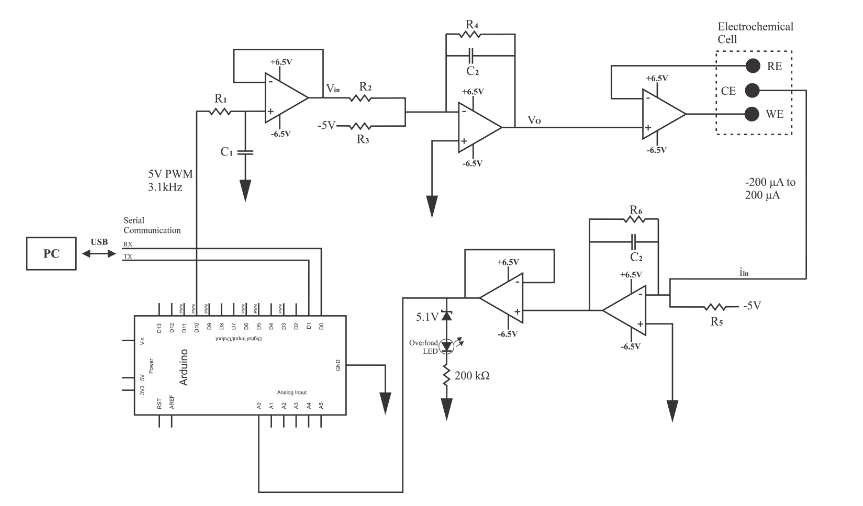
\includegraphics[width=.9\linewidth]{meloni_design.png}
\caption{Meloni Design}
\end{figure}




There are three design components that are being adjusted from the Meloni Design. First, we changed how the control signal is generated. The Meloni Design uses a single PWM pin from the Arduino in combination with an RC filter and an op-amp in an integrator configuration to produce the control signal for the CV. For our design, we chose to use a 10-bit Digital-Analog Converter (DAC) using an R2R ladder. This offers two benefits: first, it offers greater resolution for the control signal - 10-bit precision instead of 8-bit with the PWM design. The R2R ladder is a fundamental circuit design used in entry-level electrical engineering coursework, whereas the PWM design may be considered more advanced. Second, we chose to swap the connections between the working electrode and the counter electrode. This design decision was made with consultation from a BioLogic representative who claimed that since we are concerned about the current through the working electrode, it is assumed that measuring the current directly through it is the optimal design solution. Third, we will change the method used for current to voltage conversion. We will use the benchmark testing current maximum and minimum values to calculate an appropriate current measuring resistor and this voltage will be buffered, amplified, and then buffered again before being sent to the Arduino for further processing.


The modifications to the original Meloni Design were made in line with theoretical circuit analysis techniques. The use of an R2R ladder and the need for future students to perform circuit analysis to attenuate component values offer a greater learning opportunity for students. With this in mind the construction of the potentiostat used in this report can be understood as follows (fig. 3).


\begin{figure}[h]
\centering
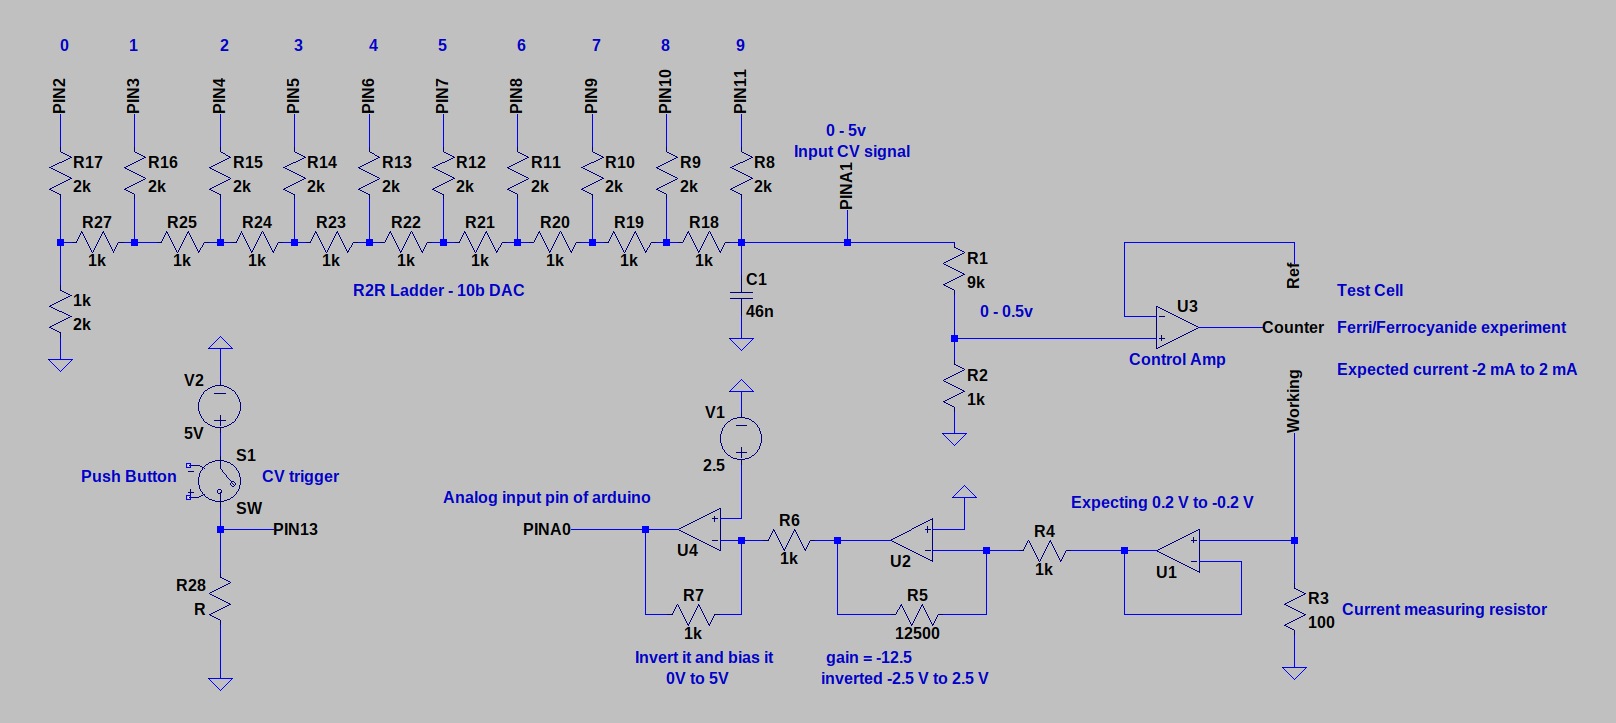
\includegraphics[width=.9\linewidth]{diy_design.png}
\caption{Our Design}
\end{figure}


\subsubsection*{Hardware Design}
For our potentiostat design we are using an Arduino Uno as the main controller of the potentiostat. Additionally, a quad operational amplifier will be the heart of the potentiostat hardware design, this will be powered by a +/- 12 volt power supply. The Arduino Uno will be responsible for outputting the CV control signal and it will be responsible for sensing the potential applied at the test cell and the output voltage to be used to calculate the output current that passes through the working electrode of the test cell. Further data processing will be conducted using serial communication between the Arduino and a computer.


The output control signal that will generate the CV begins with the Arduino's digital pins 2-11. These pins are connected to a corresponding 10 bit R2R ladder which acts as the potentiostats DAC. Since the digital output of each pin is 5 volts the possible output of this R2R ladder will range from 0 to 5 volts. In order to get an accurate reading of the potential being applied to the control amplifier, the Arduino will be sensing the voltage at the output of this R2R ladder, which is connected to the Arduino's analog input pin A1.


The next stage we will process the signal to fit within the desired potential range. For our experiment we are using a CV potential range from 0v to 0.5v. This can be achieved using a voltage divider to scale the control signal by one tenth. It should be noted that this value can be adjusted to fit other potential ranges depending on the needs of future researchers. This scaled signal is then fed to the non-inverting input terminal of the control amplifier.


The output of the control amplifier is connected to the counter electrode of the test cell, while the reference electrode is connected to the inverting input of the control amplifier. The control amplifier is the heart of the potentiostat. This element is what ensures that the voltage at the reference electrode follows the control signal. The working electrode is then connected to a measurement resistor which is then connected to ground.


This voltage is then scaled to fit within the Arduino's 0 to 5 volt sensing range. It is important to note that the scaling function and component values may need to be adjusted depending on the voltage that is detected across the measurement resistor. It is crucial that the signal can fit well within this range, if not, then the signal will become clipped and experimental data will be lost.


For our experiment we expect a current within the bounds of -2mA to 2mA. This will then be amplified using an op amp in an inverting amplifier configuration and then the signal will be inverted again and biased to fit within the 0 to 5 volt range of the Arduino sensing range. We will see in the results that this configuration will be adjusted due to errors in the experimental set up.


In addition to the potentiostat circuit, there is also a push button that is used to initialize the CV experiment. This takes a 5v signal from the Arduino, passes it to a button, which then completes a circuit through a resistor to ground, when the 5v is sensed it will begin the CV sweep.


\begin{figure}[H]
\centering
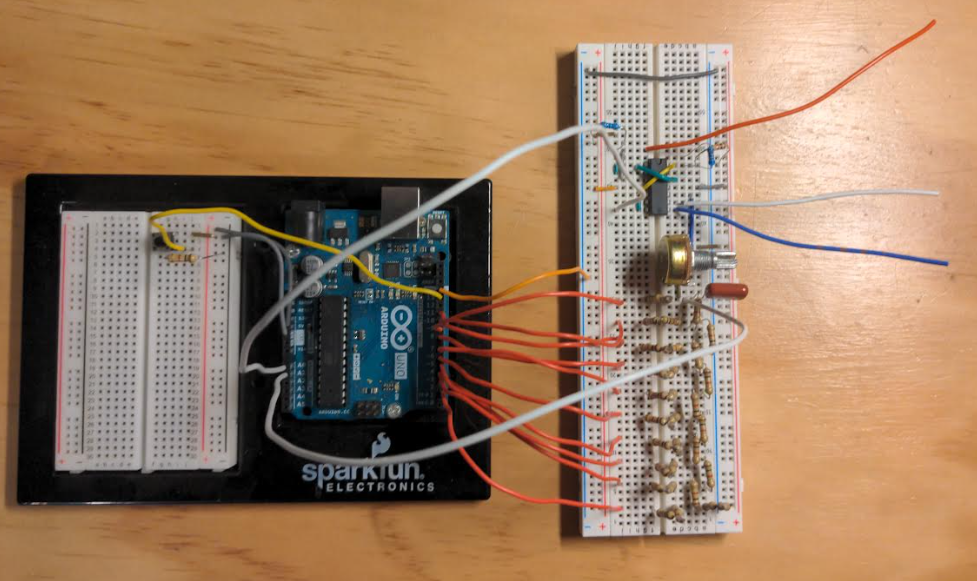
\includegraphics[width=.9\linewidth]{hardware_design.png}
\caption{Hardware Design | The red, white, and blue wires connect to the Working, Reference, and Counter electrodes respectively.}
\end{figure}


\subsubsection*{Software Design}


The software design has two core components: the CV function and data processing. The CV function consists of two parts, the C++ Arduino code and a python script to capture serial transmission data from the Arduino. The data processing step will take the recorded data, process it and output the CV graph and data.


The Arduino code presents a functional potentiostat software tailored for conducting CV measurements. The sketch operates in a loop, waiting for a trigger signal to activate the CV mode. Within the CV mode, the \texttt{cvMode} function controls the voltage output to the potentiostat based on elapsed time and a specified scan rate, generating the desired waveform. The function employs a while loop to execute a series of CV cycles until the desired cycle count is reached. During each cycle, the sketch reads voltage output from the potentiostat and the electrochemical cell's response using analog-to-digital converters. Real-time data is printed to the Serial Monitor, allowing researchers to monitor the CV operation. The sketch can be extended for other electrochemical studies, offering a versatile tool for exploring redox behavior in materials. (See Appendix 1 for source code)


The Python script facilitates real-time data acquisition via the Arduino's USB serial connection. Upon establishing the serial port configuration, the script enters a continuous loop to read data from the potentiostat. The acquired data is written to a text file enabling the accumulation of results. The script is designed to run indefinitely until interrupted by a keyboard interrupt. This script provides a convenient means of acquiring and saving data. (See Appendix 2 for source code)


Finally, there is the data processing software. This consists of a Python script which takes the collected data from a text file. It first parses the text file and then performs a conversion of the data to conform to the values we are looking to measure. This data is then output to a text file and the CV graph itself. The process of converting the sensor data into their corresponding values for either potential or current rely heavily on the researchers hardware design choices. The analog input sensors on the Arduino Uno detect voltage values from 0 to 5 volts and convert the analog signal to a digital signal with 10-bit precision. This means that for both measurements we must convert a value between 0 - 1023 to fit either potential (for the input signal) or current (for the output signal).


For our experiment the input voltage must be converted from steps (0 - 1023) to volts (0 - 0.5) and the output current must be convert from steps (0 - 1023) to volts (0 v - 5 v) and then to current (-2.5 mA - 2.5 mA). To tackle the input voltage we will take the value in steps, multiply by 5 and divide by 1023, to convert from steps to volts. Then divide again by 10 to account for the voltage divider in our circuit. To convert the sensor data from steps to current requires a little more work. Due to the errors in current measurements that will be discussed later in this report we had to shift the design to accommodate that limited current range. The process of converting the current is as follows - divide by 1023 and multiply by 5 to convert from steps to voltage. Then divide by 69.3 (the amplification factor used to boost the signal in the hardware design). This will give us the voltage across the measurement resistor, to get current we will divide by 100, the value of the measurement resistor. This will then be converted to milliamps by multiplying by 1000. (see Appendix 3 for source code)


\begin{align*}
  V_{\text{{input}}} = \frac{{\text{{steps}} \times 5}}{{1023 \times 10}} \qquad \qquad 
  V_{\text{{output}}} & = \frac{{\text{{steps}} \times 5}}{{1023}} \\
  V_{\text{{resistor}}} & = \frac{{V_{\text{{output}}}}}{{69.3}} \\
  I_{\text{{output}}} & = \frac{{V_{\text{{resistor}}}}}{{100}} \times 1000
\end{align*}

\subsubsection*{Benchmarking: Ferri/Ferrocyanide Redox Reaction Electrochemical Cell Setup}

The electrochemical reaction to be studied is a ferricyanide/ferrocyanide redox reaction. This reaction will first be conducted using a BioLogic VSP-300 potentiostat using the EC-Lab software. A CV will be produced using a potential window from 0 to 0.5 volts, with scan rates of 20, 50, and 100 mV/s for 5 cycles each. This benchmark testing will also provide an expected current range of the redox reaction. The same experimental procedure will be conducted using our DIY potnetiostat.

For the complete experimental procedure and electronics lab companion see the Supplemental Material section.


\subsection*{Results and Discussion}

During testing of our DIY potentiostat against a BioLogic VSP-300 potentiostat, the measured current response from the working electrode displayed discernible trends. The current fluctuated within the ranges of 0 to 0.4 volts, 0 to 0.5 volts, and 0 to 0.6 volts for scan rates of 20 mV/s, 50 mV/s, and 100 mV/s, respectively (Figure 5). However, a notable disparity emerged when compared to the BioLogic potentiostat's measurements, with the absence of the expected `duck shaped' cyclic voltammogram.

\begin{figure}[H]
\centering
\begin{subfigure}[b]{0.45\textwidth}
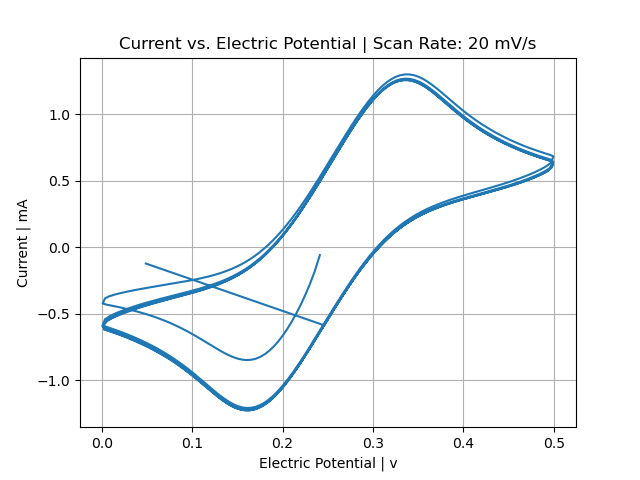
\includegraphics[width=\textwidth]{FECN_20mVs_5cycles_lab.png}
\caption{BioLogic VSP-300 FeCN 20 mV/s 5 cycles}
\end{subfigure}
\hfill
\begin{subfigure}[b]{0.45\textwidth}
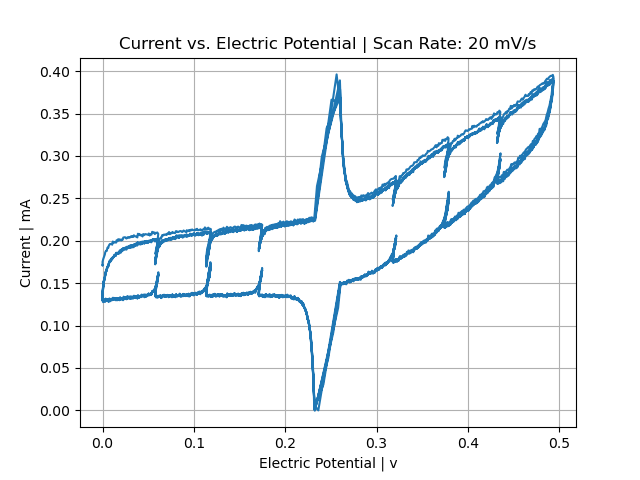
\includegraphics[width=\textwidth]{FECN_20mVs_5cycles.png}
\caption{DIY Potentiostat FeCN 20 mV/s 5 cycles}
\end{subfigure}

\begin{subfigure}[b]{0.45\textwidth}
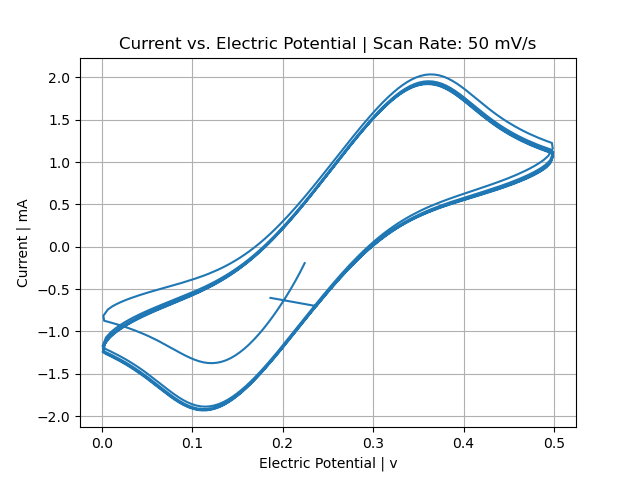
\includegraphics[width=\textwidth]{FECN_50mVs_5cycles_lab.png}
\caption{BioLogic VSP-300 FeCN 50 mV/s 5 cycles}
\end{subfigure}
\hfill
\begin{subfigure}[b]{0.45\textwidth}
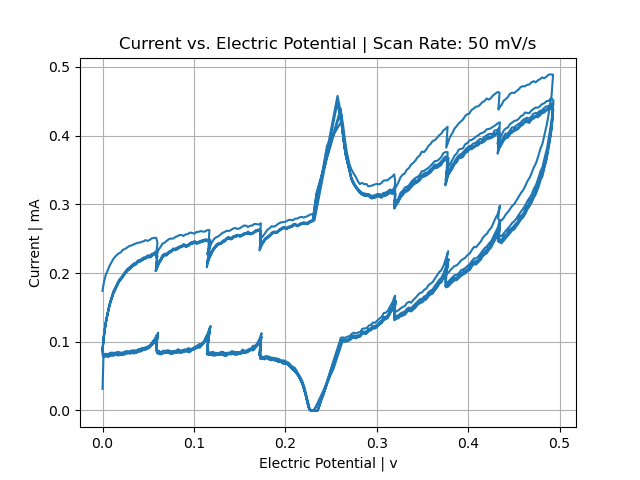
\includegraphics[width=\textwidth]{FECN_50mVs_5cycles.png}
\caption{DIY Potentiostat FeCN 50 mV/s 5 cycles}
\end{subfigure}

\begin{subfigure}[b]{0.45\textwidth}
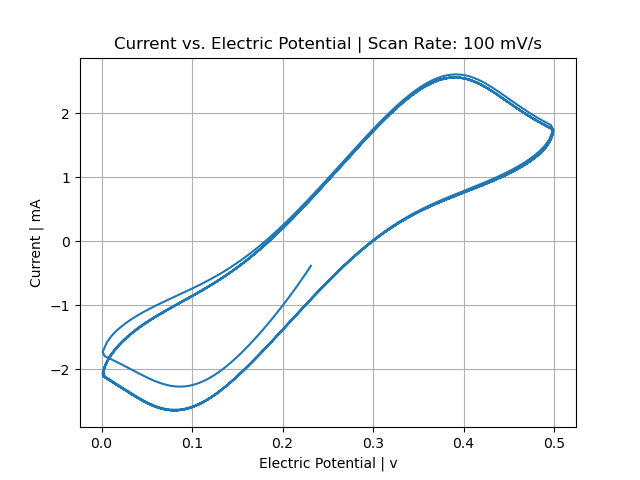
\includegraphics[width=\textwidth]{FECN_100mVs_5cycles_lab.png}
\caption{BioLogic VSP-300 FeCN 100 mV/s 5 cycles}
\end{subfigure}
\hfill
\begin{subfigure}[b]{0.45\textwidth}
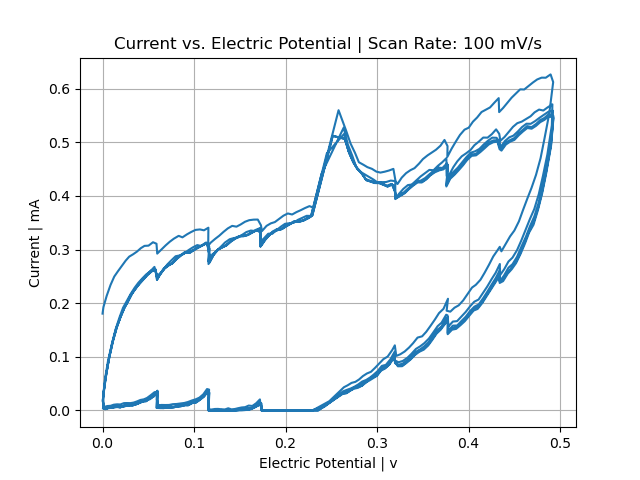
\includegraphics[width=\textwidth]{FECN_100mVs_5cycles.png}
\caption{DIY Potentiostat FeCN 100 mV/s 5 cycles}
\end{subfigure}
\caption{Side-by-side comparison of cyclic voltammograms}
\end{figure}


The consistency observed in the current response, despite the disparity with the expected cyclic voltammogram, reveals complex dynamics within the potentiostat's function. The discrepancy may point to a limitation or error in the potentiostat design itself. When analyzing the data collected from the DIY potentiostat we see noteable events occuring at approximately 0.07 v, 0.12 v, 0.18 v, 0.23 v, 0.28 v, 0.32 v, 0.38 v, and 0.43 v. These events show characteristics of capacitor charging and rapidly discharging events. This occurs at the near the same potential despite the scan rate. Several factors might have contributed to these unexpected results.

Extensive hardware troubleshooting was conducted. Each signal processing step within the hardware was tested using signals in the expected range of the electrochemical cell. In isolated testing scenarios, the hardware produced the expected values. The success in isolated hardware testing adds complexity to the observed limitation in the current range when connected to the actual electrochemical cell. The divergence between the isolated testing and real-world application highlights a critical area of investigation.

\begin{figure}[H]
  \centering
  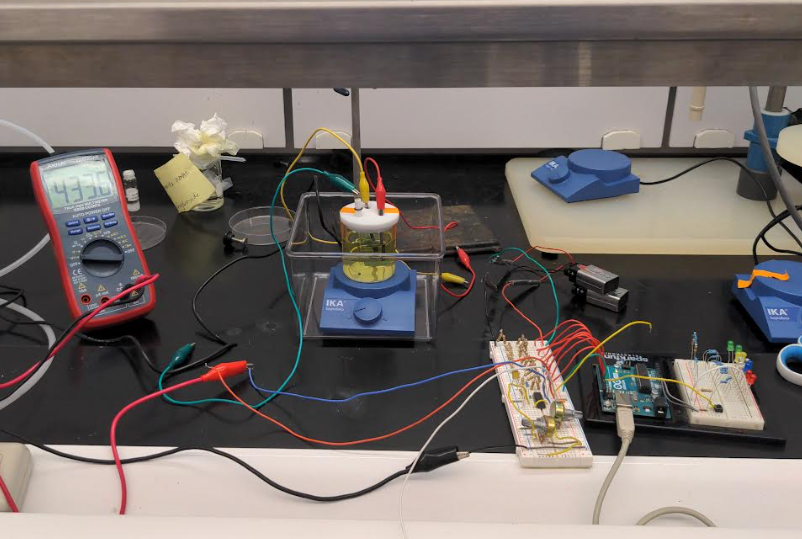
\includegraphics[width=.9\linewidth]{lab_test.png}
  \caption{Ferri/ferrocyanide Redox Reaction Test}
  \end{figure}
  

Though the hardware was designed according to specifications, the observed limitations may stem from several potential sources.
\begin{enumerate}
\item \textbf{Poor Hardware Design}: The entire architecture might not have been optimal for the specific application, leading to inherent limitations.
\item \textbf{Component or Breadboard Issues}: The use of specific components or the breadboard itself might have introduced unexpected behaviors or constraints.
\item \textbf{Choice of Operational Amplifier}: The chosen operational amplifier (LT074 Op Amp) for the design may not have been suitable as the control amplifier.
\end{enumerate}

The multifaceted nature of the potential errors presents a challenge in pinpointing the exact cause. Further detailed analysis and redesign may be required to isolate and rectify the underlying issues. The findings from this study provide valuable insights into the complexities of custom potentiostat design. While the observed trends and successful isolated testing demonstrate a degree of functionality, the disparity with expected results points to critical areas for improvement.

Further investigation into the specific components, hardware design, and choice of operational amplifier is warranted. Future work should focus on systematically evaluating each potential source of error, leading to refined designs and potentially unveiling insights into potentiostat function.



Despite existing errors in our DIY potentiostat design, this research highlights potential success with our expressed goal of developing educational materials and tools. With further time and assistance from electrical engineering professionals, achieving a DIY design that rivals lab-grade instruments may be possible.

\subsection*{Conclusion}
The aim of this project was to consolidate existing research on cost-effective potentiostat designs and create a comprehensive educational resource for students engaging in electrochemical engineering research. While the final iteration of our design did not meet the benchmarking standards necessary to replace lab instruments, the process yielded valuable educational insights.

The developed DIY potentiostat demonstrated a consistent systematic error pattern rather than random variability. Although it may not be suitable for conducting precise experiments, it lays the foundation for deeper exploration and hardware calibration. This opens up opportunities to refine the DIY potentiostat design and align it more closely with benchmarking criteria. By following the lab procedures in the supplemental materials sections and with appropriate guidance, students can gain valuable educational insights with respect to electrochemistry and electrical engineering.

\subsection*{Acknowledgments}

We express our gratitude to Intel for providing the funding to Oregon State University for this research internship. Their generous support has been pivotal in enabling this work.


Special thanks to Dr. Kelsey Stoerzinger, who not only served as the main professor and mentor but also facilitated access to her lab where the research was conducted. Her guidance, expertise, and encouragement have been invaluable to the success of this project.


We are also deeply indebted to Dr. Stoerzinger's graduate and postdoctoral students: Sri Krishna Murthy Padavala, Jorin Dawidowicz, Kelly White, Molly Vitale-Sullivan, and Rajkumar Jana. Their support, hands-on assistance, and insightful feedback have greatly enriched this work.

Additionaly, we would like to thank Dr. Neil Spinner and his colleauges from Pine Research for their responsiveness to our requests for assistance. 

Lastly, we acknowledge the entire team at OSU and all those who contributed directly or indirectly to this research, for creating an environment conducive to innovation and discovery.


\subsection*{References}
Butterworth A, Corrigan DK, et al. (2019) Electrochemical detection of oxacillin resistance with SimpleStat: a low cost integrated potentiostat and sensor platform. \emph{Analytical Methods.} Issue 14.


Cook J (2020). SIMstat: Hardware Design Considerations for Implementing a Low-Cost, Portable Potentiostat. \emph{Unpublished Bachelor's Thesis}. Oregon State University


Cordova-Huaman AV, Jauja-Ccana VR, et al. (2021) Low-cost smartphone-controlled potentiostat based on Arduino for teaching electrochemistry fundamentals and applications.\emph{Heliyon}, Volume 7, Issue 2.


Meloni, GN (2016). Building a Microcontroller Based Potentiostat: A Inexpensive and Versatile Platform for Teaching Electrochemistry and Instrumentation. \emph{Journal of Chemical Education} 93(7), 1320-1322.


Rowe AA, Bonham AJ, et al. (2011) CheapStat: An Open-Source, ‘‘Do-It-Yourself’’ Potentiostat for Analytical and Educational Applications. \emph{PLoS ONE} 6(9).


\newpage
\section*{Supplemental Material}
\subsection*{FeCN Measurement}
\subsubsection*{Background on the Importance of Measurement and Objective:}
An outersphere redox couple changes oxidation state via electron transferto/from an electrode surface. This has some associated reversible potential:
\[ [Fe^{|||}(CN)_6]^{3-} + 1e^- \leftrightarrow [Fe^{||}(CN)_6]^{4-}\]
If you have a mixture of these two salts and hold the working electrode below this potential (smaller/negative voltages), ferricyanide will be reduced, giving a negative current. Above it, ferrocyanide will be oxidized, giving a positive current. The current will initially be high in magnitude (due to some charging current and the presence of reactants near the surface) and decay to some steady state value (which reflects how quickly the reactant can diffuse to the electrode surface). We often measure such reactions by cyclic Voltammetry where the voltage is swept at a given scan rate ($v$), turning this profile into a characteristic duck-like shape. The Randles Sevick equation describes the effect of $v$ on the peak current ($I_p$) for a reversible process:
\[ I_p = (2.69*10^5) AD^{0.5}Cv^{0.5}\]
Where $A$ is the electrode surface area ($cm^2$), $D$ is the diffusion coefficient ($\frac{cm^2}{s}$) and $C$ is the concentration of electroactive species in the bulk solution ($\frac{mol}{cm^3}$).
\subsubsection*{Safety}
Understand the hazards of the electrolyte you are using and review any pertinent SDSs; secondary containment is suggested in case of spills. Note that ferri/ferrocyanide should not be used in acidic electrolyte as this can cause cleavage of the -CN groups, yielding a toxic gas. Performed in the range around the reversible potential suggested here the experiment should be fine to perform without ventilation, but it's suggested to perform the experiment in the hood for added caution.


\subsubsection*{Materials}
\begin{itemize}
\item Clean glass (neutral or alkaline electrolyte) or PTFE (alkaline) electrochemical cell (see glassware cleaning SOP)
\begin{itemize}
\item Note: Fe is notorious for diffusing into glass and gives it a yellow hue that is nearly impossible to remove. Please perform experiment in a designated cell.
\end{itemize}
\item 2 clean graphite rod (or other working and counter electrodes)
\item 1 clean sparge bar, or pipette tip on gas line (suggested)
\begin{itemize}
\item Note: Fe is notorious for diffusing into glass and gives it a yellow hue that is nearly impossible to remove. Please perform experiment in a designated cell.
\end{itemize}
\item Reference electrode. Be sure to rinse this copiously with Millipure water as they are stored in salt solution (e.g. hold under flow while rotating for a few seconds).
\item Clean stir bar and stir plate
\item Potentiostat
\end{itemize}
\subsubsection*{Procedure}
\begin{enumerate}
\item Prepare your electrolyte (suggestion: 0.1 M KOH + 5 mM each of Fe(III) and Fe(II) salts) within your electrochemical cell. Use Millipure water (make sure the reading is 18.2 M$\Omega$), measuring volume with a graduated cylinder marked for water only. Add required salts and mix. Note all details in your lab book.
\begin{itemize}
\item Suggestion: KOH is in big pellets; measure this first, then calculate how much Fe(III), Fe(II) and water you need to hit the desired composition.
\end{itemize}
\item Begin sparging and stirring the electrolyte volume with $N_2$. The objective is to displace $O_2$, which will give an additional Faradaic current (from the oxygen reduction reaction). The smaller the bubbles the quicker this will happen. Note the time in your lab book (do this for ~30 minutes).
\item Secure the electrodes within your cell. Some fit nicely via holders/O-rings, others you balance with an electrochemical clip or affix with lab tape.
\item Connect the lab potentiostat leads, being careful not to short them or touch any metal to them.
\begin{itemize}
\item Working Electrode: Carbon rod (or otherwise)
\item Counter Electrode: Carbon rod (or otherwise)
\item Reference Electrode: Ag/AgCl reference electrode
\end{itemize}
\item Perform a CV 0 volts to 0.5 volts at scan rates of 20, 50, and 100 $\frac{mV}{s}$ for 5 cycles each without stirring. Note the expected maximum and minimum current range to attenuate DIY potentiostat current to voltage conversion.
\item Attenuate current to voltage components in hardware to fit adequately read the expected current.
\item Disconnect the lab potentiostat and reconnect it to the DIY potentiostat. Conduct the experiment again, recording each scan rate for 5 cycles each.
\end{enumerate}
\subsubsection*{References}
\begin{itemize}
\item https://pubs.acs.org/doi/pdf/10.1021/ed200604m
\item https://pubs.acs.org/doi/pdf/10.1021/ed073p808
\end{itemize}
\newpage
\section*{Appendix}
\subsubsection*{1}
\begin{lstlisting}
// Christopher Hunt
// potentiostat.ino


// User Set Init Params
const int CELL_OUTPUT = A0; // Analog Read pin to read electrochemical cell output. Reads voltage data from TIA in circuit.
const int CV_VOLTAGE = A1; // Reads current voltage being supplied to the potentiostat.
const uint8_t TRIGGER_PIN = 13; // Trigger pin. Detecting push button to trigger the CV.
const int MODE = 0; // Mode 0 is CV. Designed to potentially expand to perform EIS
// Cyclic Voltammetry : mode = 0
const float SCAN_RATE = .1; // The rate of the CV scan in V/s
const int CYCLES = 50; // How many times the CV is performed
/**
* Function: cvMode
* ----------------
* Implements the CV (Cyclic Voltammetry) mode of operation. The function performs a series
* of CV cycles until the specified number of cycles (CV_CYCLES) is reached. It controls the
* voltage output based on the elapsed time and scan rate, updating the DAC ports to generate
* the desired waveform.
*
* The function utilizes a while loop to execute the CV cycles until the cycle count reaches
* the desired number of cycles. It maintains the elapsed time since the start of the CV mode
* using the `micros()` function. By comparing this elapsed time with the scan rate and direction,
* it calculates the corresponding voltage value (`value`) for the DAC ports.
*
* The function employs an if-else statement to determine whether the voltage should increment
* or decrement based on the current direction (`forward`). The `adj_scan_rate` is used to adjust
* the rate of change per unit time. If the calculated value exceeds the range of 0 to 1023,
* it is clamped to the corresponding limit, and the direction is switched accordingly.
*
* The function then calls the `portSelectDAC` function to configure the DAC ports with the
* calculated voltage value. The DAC value is split into two bytes (`portdb_bytes[0]` and `portdb_bytes[1]`),
* which are then assigned to the appropriate DAC ports. This enables the generation of the desired waveform.
*
* Additionally, the current `value` is printed to the Serial Monitor using `Serial.println()`,
* providing real-time feedback and monitoring of the CV operation.
*/
void cvMode() {
const float scan_rate = SCAN_RATE * (10230.0 / 5000000.0);
bool forward = true;
int cycle = 0;
unsigned long start_time = micros();
unsigned long time = 0;
float value = 0;
int rounded_value = 0;
int sensor_value = 0;
int control_value = 0;
unsigned long last_read_time = 0;
const unsigned long read_interval = 1000; // Microseconds between reads
while (cycle < CYCLES) {
time = micros() - start_time;
if (forward) {
value = scan_rate * time;
rounded_value = (int)value; // Typecast directly to int
if (rounded_value >= 1023) {
rounded_value = 1023;
forward = false;
start_time = micros();
}
} else {
value = -scan_rate * time + 1023;
rounded_value = (int)value; // Typecast directly to int
if (rounded_value <= 0) {
rounded_value = 0;
forward = true;
start_time = micros();
cycle++;
}
}
// Send value to 10-bit DAC
PORTD = (rounded_value << 2) & 0xFC;
PORTB = (rounded_value >> 6) & 0x0F;
// Calculate average and send data every read_interval2 microseconds
if (micros() - last_read_time >= read_interval) {
last_read_time = micros();
control_value = analogRead(CV_VOLTAGE);
sensor_value = analogRead(CELL_OUTPUT);
Serial.print(control_value);
Serial.print('\t');
Serial.println(sensor_value);
}
}
}
/**
* Function: setup
* ----------------
* Configures the initial setup and pin modes for an Arduino sketch.
* It sets the data direction registers (DDRx) for digital pins D2 to D7 and B0 to B3,
* configures pin C0 as an input pin, and initializes the Serial communication at 9600 baud rate.
*
* Pin Configuration:
* - Digital pins D2 to D7 are set as output pins by setting the corresponding bits in DDRD to HIGH (1).
* - Digital pins B0 to B3 are set as output pins by setting the corresponding bits in DDRB to HIGH (1).
*
* Serial Communication:
* - Serial communication is initiated by calling `Serial.begin(9600)`.
* - The baud rate is set to 9600 bits per second.
*/
void setup() {
DDRD |= B11111100;
DDRB |= B00001111;
pinMode(CELL_OUTPUT, INPUT);
pinMode(CV_VOLTAGE, INPUT);
// Set pins to 0v
PORTD = 0x00;
PORTB = 0x00;
Serial.begin(9600);
}
/**
* Function: loop
* ----------------
* The main execution loop for the Arduino sketch.
* It waits for the trigger pin to go HIGH and then executes the selected mode based on the MODE variable.
* After completing the mode execution, it waits for a specified delay before starting the sequence again.
*
*/
void loop() {
// Wait for trigger pin to go HIGH
while (digitalRead(TRIGGER_PIN) == LOW) {
}
switch (MODE) {
case 0:
cvMode();
break;
default:
Serial.print("Incorrect Mode.");
break;
}
// Wait before starting the sequence again
delay(1000); // Adjust the delay between repetitions as needed
}
\end{lstlisting}


\newpage\subsubsection*{2}
\begin{lstlisting}
# Christopher Hunt
# serial_2_txt.py
import serial
import sys


# Serial port configuration
serial_port = '/dev/ttyACM0' # Replace with the appropriate serial port
baud_rate = 9600


# File path for saving data
file_path = 'data.txt'


# Open the serial port
ser = serial.Serial(serial_port, baud_rate)


# Open the file in append mode
with open(file_path, 'a') as file:
try:
# Read data from the serial port and write it to the file
while True:
if ser.in_waiting > 0:
data = ser.readline().decode().strip()
file.write(data + '\n')
file.flush() # Flush the buffer to ensure immediate writing


except KeyboardInterrupt:
# Handle keyboard interrupt (Ctrl+C)
print("Keyboard interrupt detected. Exiting...")
ser.close() # Close the serial port
sys.exit(0)


\end{lstlisting}


\newpage
\subsubsection*{3}
\begin{lstlisting}
import matplotlib.pyplot as plt
import argparse
def parse_data(file_path):
"""
Parses data from a file and extracts x and y values for plotting.
Parameters:
file_path (str): The path to the data file.
Returns:
tuple: A tuple containing two lists. The first list contains the parsed x values,
and the second list contains the parsed y values.
"""
in_voltage_transfer_func = 5 / (10 * 1023)
out_voltage_transfer_func = (5 * 1000) / (69.3 * 1023 * 100)
x_values = []
y_values = []
with open(file_path, 'r') as file:
for line in file:
data = line.strip().split('\t')
if len(data) == 2:
data[0] = in_voltage_transfer_func * float(data[0])
data[1] = out_voltage_transfer_func * float(data[1])
x_values.append(data[0])
y_values.append(data[1])
x_values = [sum(x_values[i:i + 5]) / 5 for i in range(0, len(x_values), 5)]
y_values = [sum(y_values[i:i + 5]) / 5 for i in range(0, len(y_values), 5)]
return x_values, y_values
# Add command-line argument parsing
parser = argparse.ArgumentParser(description='Plot data from a file.')
parser.add_argument('data_file', type=str, help='Path to the data file.')
parser.add_argument('scan_rate', type=int, help='Scan Rate of CV')
args = parser.parse_args()
# Use the data file path provided as a command-line argument
data_file = args.data_file
scan_rate = args.scan_rate
x, y = parse_data(data_file)
# Save the new data to a file named "new_data.txt"
with open(f'FECN_{scan_rate}mVs_5cycles_data.txt', 'w') as file:
for i in range(len(x)):
file.write(f"{x[i]}\t{y[i]}\n")
# Plot the graph and save it to "graph.png"
plt.plot(x, y)
plt.xlabel('Electric Potential | v')
plt.ylabel('Current | mA')
plt.title(f'Current vs. Electric Potential | Scan Rate: {scan_rate} mV/s')
plt.grid(True)
plt.savefig(f'FECN_{scan_rate}mVs_5cycles.png')
\end{lstlisting}


\end{document}

